%!TEX root = ./../main.tex
\section{Convolutional Neural Network}
Ein neuronales Netz entspricht dem Modell eines menschlichen Gehirns. Wie der Name schon sagt, werden die Funktionen von Nervenzellen, auch Neuronen genannt, simuliert. Ein solches Netz kommt dann zum Einsatz, wenn die Grenzen der Algorithmik erreicht sind und komplexe Aufgaben einen gewissen Grad an Generalisierung erfordern. Diese Netze kommen in den unterschiedlichsten Anwendungsgebieten zum Einsatz: 
\begin{itemize}
  \item Bild -bzw. Mustererkennung (inkl. des Erkennens von Sprache und Handschrift)
  \item Finanzanalyse
  \item Diagnose in der Medizin
  \item Unterstützung bei Entscheidungen, Planungsaufgaben und bei der Qualitätskontrolle
\end{itemize}
Neuronale Netze sollen die herkömmliche Technologie nicht ersetzen, sondern diese ergänzen und deren Schwächen ausgleichen. Schwächen wie zum Beispiel bei Szenarien mit verrauschten, fehlerhaften oder vagen und unvollständigen Daten\cite{Kaffka.2017}.\\
Unter den neuronalen Netzen gibt es eine Vielzahl an Spezialisierungen welche sich auf eines oder mehrere der oben genannten Anwendungsgebieten festgelegt haben. Eines davon ist das CNN (dt. faltendes neuronales Netzwerk). Dieses eignet sich am besten für die Bearbeitung und Klassifizierung von Bildern.\\
Bei der Klassifizierung geht es darum, aus einem Eingabebild eine entsprechende Klasse (bspw. Hund, Katze etc.) oder auch Wahrscheinlichkeiten der am ehesten zutreffenden Klassen abzuleiten. Um solche komplexen Aufgaben meistern zu können, orientiert sich das CNN an dem Aufbau und der Funktionsweise eines visuellen Kortexes.\\
Dieser besteht aus kleinen Neuronengruppen, die auf bestimme Bereiche des Sichtfeldes empfindlich reagieren. Darunter gibt es für bestimmte Anordnungen von Kanten wie z.B. horizontale, vertikale oder diagonale Kanten unterschiedliche Neuronen, welche stimuliert werden sobald diese Anordnung in deren Nähe auftritt. Diese Vorgehensweise, dass spezielle Komponenten in einem System spezielle Aufgaben haben, in diesem Fall Neuronen, welche auf bestimmte Charakteristika reagieren, wird auch von Maschinen benutzt und stellt die Basis von CNNs dar.

\subsection{Schichten}
Ein CNN besteht aus einer Serie von unterschiedlichen Schichten, auch Netzarchitektur genannt siehe Fig.~\ref{fig-architecture}.
\begin{figure*}[htbp]
\centerline{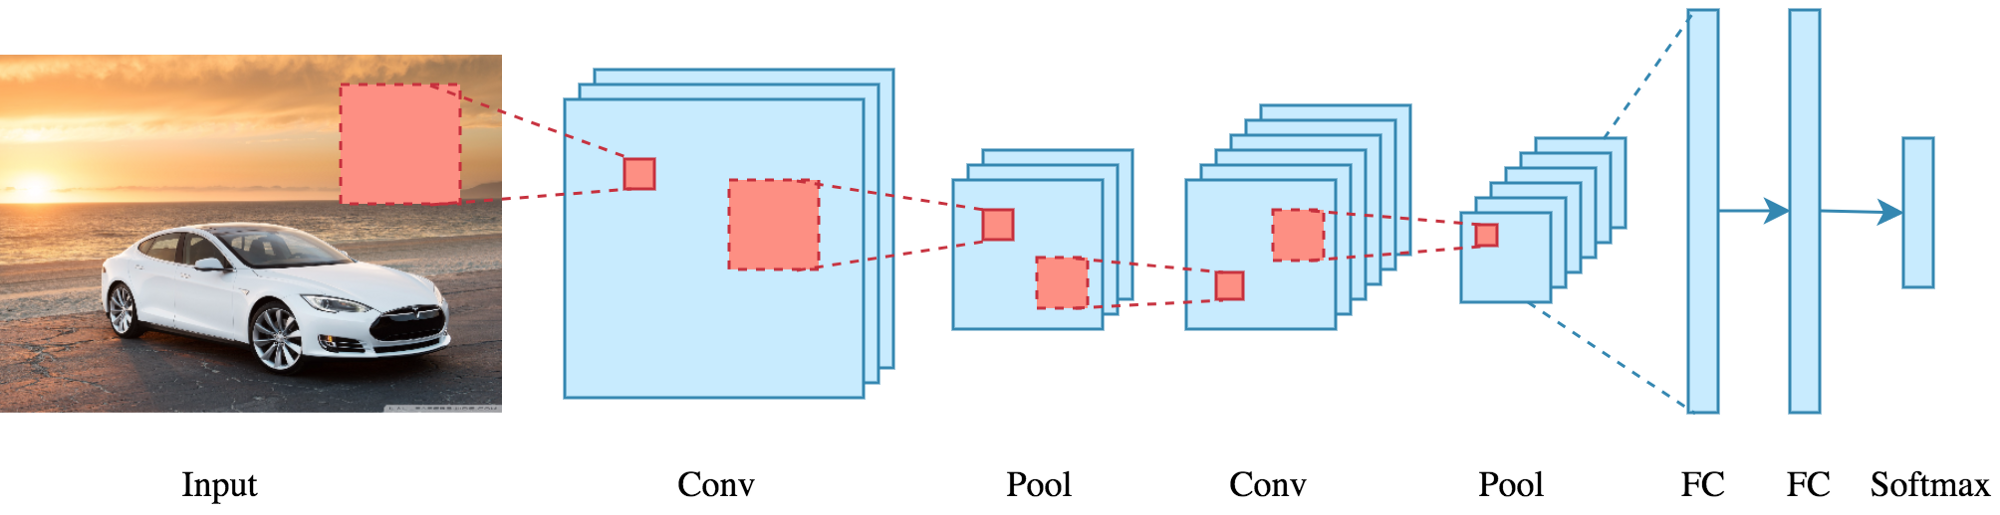
\includegraphics[height=3.3cm]{img/architecture-cnn-car.png}}
\caption{Netzarchitektur \cite{Dertat.2017}}
\label{fig-architecture}
\end{figure*}

\subsubsection{Input-Schicht}
Das ist die erste Schicht der Architektur, bei welcher das zu klassifizierende Bild angelegt wird. Ein Bild besteht aus folgendem Volumen $Hoehe*Breite*Tiefe$, wobei die Tiefe dem Farbraum bspw. RGB entspricht. Zu beachten ist, dass die Pixelgröße durch zwei teilbar sein sollte, um bei der weiteren Verarbeitung keine Pixel zu verlieren\cite{Doukkali.2017}.

\subsubsection{Convolutional-Schicht}
Die Convolutional-Schicht ist die Namensgebende Schicht und verantwortlich für die Erkennung von Features. Features sind im übertragenen Sinne Eigenschaften von Klassen und werden in Form von Filtern dargestellt. Filter erkennen je nach Komplexitätsgrad einen Bestandteil einer Klasse und können einfachere Features miteinander verknüpfen.\\
Beispiel:
\begin{itemize}
  \item Klasse: Katze (besteht aus komplexeren Features)
  \item Feature: Kopf (besteht aus einfacheren Features)
  \subitem Auge \(\Rightarrow\) Kreisen \(\Rightarrow\) Teilkreisen \(\Rightarrow\) Rundung
  \subitem Ohr \(\Rightarrow\) Ecken \(\Rightarrow\) Geraden \(\Rightarrow\) Strich
\end{itemize}
Wichtig zu verstehen ist, dass das Netzwerk nicht wirklich weiß was ein Kopf einer Katze ist, sondern lediglich dessen strukturelle Zusammensetzung bekannt ist.\\
Ähnlich wie bei einem visuellen Kortex wendet das CNN systematisch von oben nach unten und von links nach rechts in einer zuvor definierten Größe und eines Abstandes den Filter bei dem anliegenden Input an, um daraus eine Aktivierungskarte zu erstellen. Diese Aktivierungskarte stellt dar, in welchem Teil des Bildes das Feature mit welchem Gewicht auftritt. Je höher das Gewicht ist, desto eher ist das gesuchte Merkmal in dem Teilabschnitt des Bildes vorhanden. In Fig.~\ref{fig-filter-moving} ist dieser Vorgang vereinfacht dargestellt. Das linke Quadrat zeigt in \textit{blau} den Input und in \textit{grün} den anliegenden Filter. Das rechte Quadrat stellt die Aktivierungskarte dar. Der anliegende Filter hat eine Größe von 3x3 Pixel und rückt nach jeder Berechnung um ein Pixel nach rechts bzw. zum Anfang der nächsten Zeile weiter. Was hierbei gut zu erkennen ist, dass der Filter bereits auf zwei Positionen angewendet worden ist. Einmal auf der Start-Position, wo das in \textit{grüne} Feld (Filter) sich ganz oben links befindet hat und auf der aktuellen Position. Dabei werden die Werte der Inputschicht mit den Werten des Filters multipliziert und anschließend addiert, woraus sich die Werte der Aktivierungskarte ergeben.\\
Die Performanz einer solchen Schicht richtet sich stark nach der Konfiguration der sogenannten \textit{Hyperparameter}. Diese erlauben es solch eine Schicht mit den folgenden Werten zu konfigurieren:
\begin{itemize}
  \item Filteranzahl: Gibt an wie viele Filter pro Convolutional-Schicht erstellt werden. Mehr Filter bedeutet ein aussagekräftigeres Model und erlaubt komplexere Klassen zu erkennen, erhöht aber auch die Gefahr für \textit{overfitting}. Bei \textit{overfitting} ist das Model zu sehr auf die Testklassen getrimmt und nicht mehr in der Lage zu generalisieren.
  \item Filtergröße: Hängt stark von dem Input und der zu erkennen Klassen ab. Gängige Filtergrößen sind 3x3, 5x5 oder auch 7x7. 
  \item Fortschritt: Um wie viele Pixel soll der Filter nach einer Berechnung weitergerückt werden - liegt standardmäßig bei 1.
  \item Padding: Wie in Fig.~\ref{fig-filter-moving} zu sehen ist, verkleinert sich die Aktivierungskarte abhängig von der Filtergröße und dem Fortschritt. Um dies zu verhindern und somit eine Vielzahl an sequentiellen Convolutional-Schichten zu ermöglichen, wird vor der Anwendung des Filters der Input mit entsprechenden Nullen gleichmäßig aufgefüllt, wie in Fig.~\ref{fig-padding} zu sehen ist. \textit{Blau} entspricht dem Input und \textit{grau} den Nullen, welche aufgefüllt werden. Da $0*X$ stets $0$ ergibt, beeinflusst das Padding die Aktivierungskarte nur soweit, dass sich die Summe der Aktivierungen auf einen größeren Bereich verteilt und somit einen höheren Detailierungsgrad ermöglicht.
\end{itemize}
\begin{figure}[htbp]
\centerline{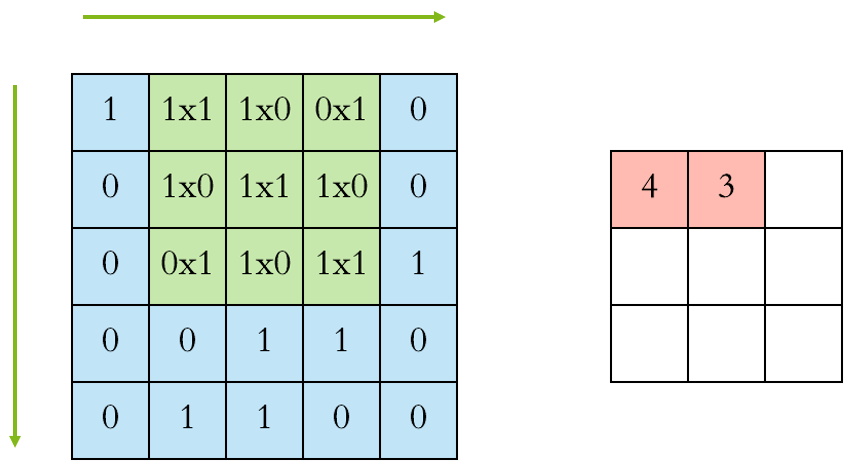
\includegraphics[height=2.9cm]{img/filter-moving.png}}
\caption{Filter convoluting \cite{Dertat.2017}}
\label{fig-filter-moving}
\end{figure}
\begin{figure}[htbp]
\centerline{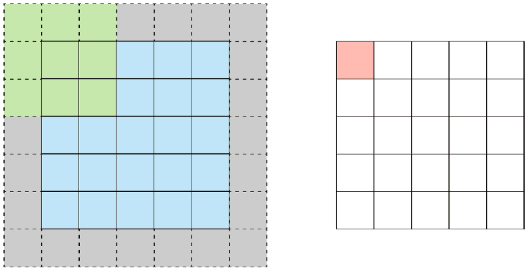
\includegraphics[height=2.4cm]{img/padding.png}}
\caption{Padding \cite{Dertat.2017}}
\label{fig-padding}
\end{figure}
Mehrere solcher Schichten hintereinander ermöglichen es komplexe Klassen zu erkennen. Die erste Schicht ist bspw. auf die Erkennung von einfachen Features, wie Kanten und Kurven spezialisiert. Die inneren Schichten sind dann schon in der Lage Halbkreise oder Kombinationen aus Kurven und Kanten bis hinzu Füße oder Flügel zu erkennen.
\subsubsection{Rectified Linear Units-Schicht}
Die Rectified Linear Units-Schicht (ReLU) muss nach Konvention direkt nach jeder Convolutional-Schicht angewendet werden um Nichtlinearität, in ein System welches nur lineare Operationen durchgeführt hat, zu integrieren. Dabei werden alle negativen Inputs mit Hilfe von der Funktion \eqref{relu} auf 0 gesetzt.
\begin{equation}
f(x)=max(0,x)\label{relu}
\end{equation}

\subsubsection{Pooling-Schicht}
Nach einer Convolutional -und einer ReLU-Schicht wird eine Pooling-Schicht angewendet um die Dimensionalität zu verringern. Dadurch kann die Anzahl der Parameter reduziert werden, was sowohl die Trainingszeit verkürzt als auch \textit{overfitting} entgegenwirkt. Die verbreitetste Pooling-Art ist das \textit{max pooling}. Hierbei wird der maximale Wert in einem festgelegten Pooling-Fenster übernommen, siehe Fig.~\ref{fig-pooling}. Zu beachten ist, dass die Größe der Aktivierungskarte halbiert wird und nur die wichtigen Informationen behalten werden, was die Anzahl der Gewichte und somit die Rechenlast stark reduzieren. Wie bei der Convolutional-Schicht wandert das Fenster über den gesamten Input, wobei die Größe und der Fortschritt konfiguriert werden können. Hierbei hat sich ein 2x2 Fenster mit einem Fortschritt von zwei Pixel bewährt\cite{Dertat.2017}\cite{.11.05.2018}.
\begin{figure}[htbp]
\centerline{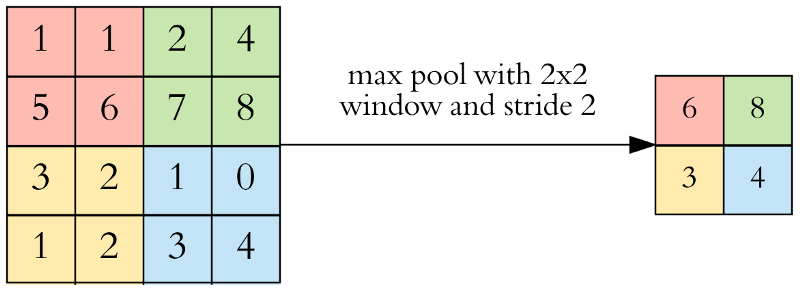
\includegraphics[height=2cm]{img/pooling.png}}
\caption{Pooling \cite{Dertat.2017}}
\label{fig-pooling}
\end{figure}

\subsubsection{Fully Connected-Schicht}
Die letzte Schicht in einer Netzarchitektur agiert als Klassifikator. Dabei werden die bereits extrahierten Features miteinander verknüpft und daraus die entsprechenden Klassen abgeleitet. Diese Schicht funktioniert wie eine Schicht aus einem klassischen neuronalen Netz, bei welcher jedes Neuron der Ausgangsschicht mit jedem der Eingangsschicht verbunden ist. Der Input der ersten Fully Connected-Schicht ist die Aktivierungskarte der vorherigen Schicht, welche die bereits extrahierten High-Level-Features beinhaltet und erkennt, welche Klasse am ehesten korreliert. Bspw. zeigt die Aktivierungskarte bei der Erkennung eines Hundes hohe Werte bei Features wie Pfoten, Füßen und eines Schwanzes.\\
Wenn mehrere Klassen erkannt werden sollen, werden die Werte der Klassen zuletzt noch mithilfe einer Softmax-Funktion in den Wertebereich $[0,1]$ transformiert um die Wahrscheinlicht ablesen zu können, siehe Fig.~\ref{fig-softmax} \cite{Deshpande.27.04.2018}.

\begin{figure}[htbp]
\centerline{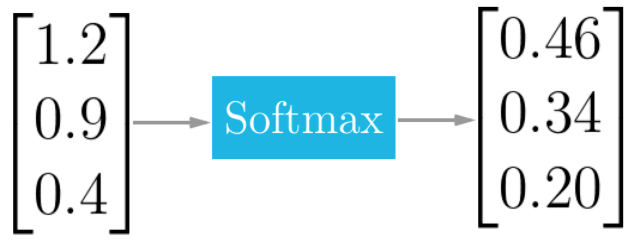
\includegraphics[height=1.2cm]{img/softmax.png}}
\caption{Softmax-Funktion\cite{JiYang.2017}}
\label{fig-softmax}
\end{figure}

\subsection{Training}
Das Training eines solchen Netzwerkes funktioniert nach dem gleichen Vorgehen, wie bei dem eines klassischen neuronalen Netzes, mithilfe von Backpropagation.\\
Dabei werden zunächst alle Gewichte des Netzwerkes mit einem zufälligen Wert belegt. Anschließend wird ein Bild, welches schon klassifiziert wurde, angelegt und durch das Netzwerk vorwärts propagiert. Dadurch bekommt man einen Output und ist in der Lage diesen mit dem Sollwert zu vergleichen um dadurch den Fehler festzustellen. Nun wird, wie der Name schon sagt, von hinten nach vorne propagiert. Dabei wird jedes Gewicht abhängig von dessen Fehlereinfluss entsprechend geändert. Die Richtung, sprich ob zu dem Gewicht etwas addiert oder etwas subtrahiert wird, wird durch das Gradient Descent-Verfahren entschieden. Bei welchem das Ziel liegt den tiefst möglichen Punkt zu erreichen. Nachdem die Richtung bekannt ist, wird das Gewicht abhängig von dessen Fehlereinfluss und der Lernrate geändert. Die Lernrate ist ein konfigurierbarer Wert, der sehr hohen Einfluss auf die Performanz eines Trainingszyklus hat. Wird diese zu hoch gewählt, springt der Fehler von einen Maximum in das nächste und ist nicht in der Lage ein akzeptables Gewicht zu finden. Wählt man hingegen eine zu niedrige Lernrate macht man nur kleine Schritte in die richtige Richtung und findet kein akzeptables Gewicht bei realistischem Rechenaufwand.\\
Dieser Vorgang wird je nach Umfang der Testdaten entsprechend oft durchgeführt, um einen bestmöglichen Grad an Generalisierung erreichen zu können\cite{Jefkine.2016}.